\documentclass[twocolumn,linenumbers]{aastex701}

\usepackage{algpseudocode}
\usepackage{xcolor}
% Numbers measured before the 2026-11-05 data and prior fixes; replace once the
% retrained networks and the corrected catalogue are in, then empty this macro.
\newcommand{\pending}[1]{\textcolor{red}{#1}}

\graphicspath{{./figures/}}
\usepackage{tikz}
\usetikzlibrary{arrows.meta,positioning}

\newcommand{\msun}{M_{\odot}}
\newcommand{\leannpe}{\texttt{LeanNPE}}
\newcommand{\dkl}{D_{\mathrm{KL}}}

\newcounter{algocount}[section]
\renewcommand{\thealgocount}{\arabic{algocount}}
\newenvironment{algorithm}[1][t]{%
  \par\addvspace{1em}\refstepcounter{algocount}%
  \noindent\hrule height 0.6pt\par\smallskip\noindent
}{%
  \par\smallskip\noindent\hrule height 0.6pt\par\addvspace{1em}%
}
\newcommand{\algcaption}[1]{\textbf{Algorithm~\thealgocount.} #1\par\smallskip\noindent}

\begin{document}

\title{LeanNPE: Rank-Conditioned Neural Posterior Estimation with an Exact Likelihood Correction for Overlapping Gravitational-Wave Signals}

\author{Bibin Thomas}
\affiliation{Otto von Guericke University Magdeburg, Germany}
\email{bibinthomas951@gmail.com}

\begin{abstract}
Next-generation gravitational-wave detectors will record compact-binary
signals often enough that two or more share an analysis segment, where a
single-signal likelihood is the wrong model and a joint sampler's cost grows
with every additional source. We present LeanNPE, an inference system built
around a rank-conditioned neural posterior estimator: from three-detector
strain and an integer rank $k$, one forward pass returns the eleven-parameter
posterior of the $k$-th loudest signal present. The network combines a
normalization-free strain encoder with an explicit inter-detector geometry
branch and a GPU matched filter over a chirp-mass template bank, whose
chirp-mass and merger-time estimates enter the normalizing flow as a pivot.
A data engine reassembles every training example from stored signal and noise
components, mixing in about 1950 segments of real LIGO--Virgo noise. The
network's posterior is the proposal of a tempered sequential Monte Carlo
sampler that evaluates the exact likelihood, with Metropolis--Hastings moves
that leave each tempered target invariant (including sky reflections and steps
along the mass-ratio--spin ridge), a higher-mode waveform, and a replicate test
that routes events it cannot resolve to nested sampling. On held-out simulated events the
binary-black-hole network \pending{[recheck after the retrain]} has near-nominal marginal coverage in all eleven parameters, in
Gaussian and real noise (90\% coverage 0.88--0.91, each $\pm0.013$ at 95\% confidence), and on thirty matched
injections its chirp-mass intervals are 1.03 times as wide as
\texttt{dynesty}'s in the median. On 28 O3 binary-black-hole events analysed
by both LeanNPE and DINGO with the same LVK noise spectra, and judged against
the published LVK posteriors, the correction moves the network's posterior from
\pending{0.75, 0.40 and 1.28} to \pending{0.17, 0.17 and 0.36} LVK standard deviations from the LVK
medians in chirp mass, mass ratio and distance, with interval widths
\pending{0.98--1.00} of LVK's; DINGO with importance sampling reaches 0.15, 0.14 and
0.48. In held-out simulations the rank-conditioned network keeps approximately
nominal marginal coverage for up to four overlapping signals, and for two
signals a joint correction agrees with joint \texttt{dynesty} posteriors in
under half an hour. We also report the architecture changes
tested to sharpen the network on loud signals, and a probe that localizes the
remaining chirp-mass precision floor in the template bank.
\end{abstract}

\keywords{gravitational waves --- methods: statistical --- methods: data analysis --- neural networks}

\section{Introduction} \label{sec:intro}

Inferring the source of a gravitational-wave detection means finding the
region of an eleven- to fifteen-dimensional parameter space consistent with
the strain, weighted by a prior. Nested sampling
\citep{Skilling2004, Speagle2020Dynesty} and Markov-chain Monte Carlo, wrapped
by \texttt{bilby} \citep{Ashton2019Bilby, Romero2020Bilby2}, do this reliably
and underlie every result in the LIGO-Virgo-KAGRA (LVK) transient catalogs
\citep{Abbott2019GWTC1, Abbott2021GWTC2, Abbott2024GWTC21, Abbott2023GWTC3}.
Their cost is $10^5$ to $10^7$ likelihood evaluations per event, minutes to
hours of wall-clock time for one signal.

That cost has been tolerable because segments containing more than one
resolvable signal have been rare. As sensitivity improves, more mergers cross
threshold per unit time, and in projected O5 and especially in third-generation
instruments a fraction of analysis segments will contain two or more signals
close enough in time to interfere \citep{Antonelli2021Overlap,
Relton2021Overlap, Samajdar2021Global, Reali2023ET}. For such data a
single-signal likelihood is not a degraded approximation but the wrong model:
it attributes the second signal's power to noise, and every parameter estimate
is measurably biased \citep{Relton2021Overlap, Janquart2023Overlap}. The
correct joint likelihood is expensive in proportion to the number of sources,
so the cost of the correct analysis grows precisely when overlaps become
common.

Amortized, simulation-based inference pays the sampling cost once, during
training. DINGO \citep{Dax2021Dingo, Dax2021Gnpe, Wildberger2023Dingo,
Dax2023DingoBns} showed that a conditional normalizing flow reaches
\texttt{bilby}-level accuracy on real LIGO events, and that importance sampling
against the likelihood corrects the network's answer and diagnoses it through
the sample efficiency \citep{Dax2023DingoBns}. These systems describe exactly one signal per segment:
the question ``which parameters explain the signal here'' has no unique answer
once a segment holds several sources.

LeanNPE answers a better-posed question: given the strain and a rank $k$, what
is the posterior of the $k$-th loudest signal present, whatever else is in the
segment? Ranks follow a deterministic loudness proxy, $\mathcal{M}^{5/6}/d_L$,
used identically in training and at inference, so no learned ordering is
involved. The contributions of this paper are:
\begin{enumerate}
\item a rank-conditioned posterior network whose encoder fuses
  normalization-free strain features, explicit inter-detector geometry, and a
  GPU matched filter over a chirp-mass template bank; the bank's estimates of
  chirp mass and merger time enter the flow as an exact shift (the
  \emph{pivot}; Section~\ref{sec:npe});
\item a data engine that reassembles every training example from stored
  signal and noise components, with real detector noise recorded between 2015 and 2025 re-colored
  exactly into each segment's measured spectrum (Section~\ref{sec:training});
\item a likelihood correction: a tempered sequential Monte Carlo sampler
  that evaluates the exact likelihood, started from the network's posterior,
  with symmetry-aware moves that leave each tempered target invariant, a
  higher-mode waveform, published power spectral densities, and a replicate
  test that hands unreliable events to nested sampling; for two overlapping
  signals the same machinery samples the 22-parameter joint posterior
  (Section~\ref{sec:correction});
\item a certification suite and three external comparisons: matched
  injections against \texttt{dynesty}, O3 events judged against the LVK
  posteriors alongside DINGO under the same noise spectra, and an
  overlap-capacity test
  (Sections~\ref{sec:setup}--\ref{sec:results});
\item a set of controlled architecture experiments aimed at the network's one
  clear weakness, chirp-mass precision on loud signals, and a probe that
  localizes it (Section~\ref{sec:experiments}).
\end{enumerate}
The central methodological point is the interplay of the last two stages: a
fast, broad amortized posterior with near-nominal coverage, and a likelihood correction
that turns it into a posterior comparable to state-of-the-art analyses, while
exposing, through replicate and \texttt{dynesty} comparisons, where the final
posterior is still unreliable.

\section{Related Work} \label{sec:related}

\subsection{Samplers}

\texttt{bilby} \citep{Ashton2019Bilby, Romero2020Bilby2} is the reference
inference framework for ground-based detectors; \texttt{dynesty}
\citep{Speagle2020Dynesty}, a nested sampler \citep{Skilling2004}, is the
sampler behind every \texttt{dynesty} comparison in this paper. Its cost is
set by how many likelihood evaluations the contraction of its live points
needs, which depends on the shape of the likelihood surface as much as on its
dimension.

\subsection{Amortized inference and importance sampling}

DINGO \citep{Dax2021Dingo} trained a conditional normalizing flow on simulated
data and reproduced \texttt{bilby}'s posteriors for real events.
\citet{Dax2021Gnpe} introduced group-equivariant NPE (GNPE), which iteratively
re-aligns each detector's data to estimated arrival times;
\citet{Wildberger2023Dingo} addressed noise-distribution shift; and DINGO-IS
\citep{Dax2023DingoBns} reweights network samples against the exact likelihood,
reporting a sample efficiency that diagnoses the network. LeanNPE's
correction differs from DINGO-IS in one essential respect: it is a tempered
sequential Monte Carlo sampler \citep{DelMoral2006Smc} whose Metropolis moves
carry particles onto the likelihood's narrow, correlated ridge, so the network
posterior need not cover that ridge itself. \citet{Green2020FlowPE}
established flow-based posterior estimation for gravitational waves; LeanNPE
uses neural spline flows \citep{Durkan2019Nsf, Papamakarios2021Flows}. These
single-signal systems were not trained or evaluated on overlapping signals.

\subsection{Overlapping signals}

Amortized inference for overlapping signals has been studied before:
\citet{Langendorff2023SBI} trained a normalizing flow on pairs of overlapping
binary-black-hole signals and showed it separates the two posteriors without
explicit subtraction. LeanNPE differs in five respects: (i) a queryable rank
replaces the fixed pair, so one network serves segments with one to four
signals; (ii) training uses real detector noise; (iii) every answer is
corrected against the likelihood; (iv) for two signals the correction samples
the joint posterior of the summed waveforms; and (v) calibration is evaluated
as a function of the number of overlapping signals, up to five. \citet{Chua2022Overlap} address
the global-fit problem of space-based detectors, where long-lived signals
overlap continuously. Studies of the bias that overlaps introduce into
single-signal analyses \citep{Antonelli2021Overlap, Relton2021Overlap,
Samajdar2021Global, Reali2023ET, Janquart2023Overlap} motivate the problem and
set the severity range we test. Machine-learning detection
\citep{Schafer2023MLGWSC, Marx2024PE} is treated here as an upstream stage.

\section{Background} \label{sec:background}

\subsection{Single-signal inference}

Detector strain for a compact-binary coalescence is $d(t) = h(t;\theta) +
n(t)$, with $n(t)$ Gaussian and stationary over one segment with one-sided
power spectral density (PSD) $S_n(f)$. The posterior is
\begin{equation}
p(\theta \mid d) = \frac{\mathcal{L}(d\mid\theta)\,\pi(\theta)}{\int \mathcal{L}(d\mid\theta')\,\pi(\theta')\,d\theta'},
\end{equation}
with the likelihood
\begin{equation}
\ln\mathcal{L}(d\mid\theta) = -\frac{1}{2}\big\langle d - h(\theta) \mid d - h(\theta)\big\rangle,
\label{eq:likelihood}
\end{equation}
and noise-weighted inner product
\begin{equation}
\langle a \mid b \rangle = 4\,\mathrm{Re}\int_0^{\infty} \frac{\tilde{a}^*(f)\tilde{b}(f)}{S_n(f)}\,df.
\label{eq:innerproduct}
\end{equation}
The optimal signal-to-noise ratio is $\rho^2 = \langle h \mid h\rangle$.
Whitening divides by the amplitude spectral density,
\begin{equation}
\tilde d_w(f) = \tilde d(f)/\sqrt{S_n(f)},
\label{eq:whitening}
\end{equation}
so that whitened noise has unit variance and the absolute amplitude of a
whitened signal is itself a loudness cue.

\subsection{Overlapping signals}

When $N$ signals share a segment, $d = \sum_i h(\theta_i) + n$, and the
correct likelihood is the joint one,
\begin{equation}
\ln\mathcal{L}(d \mid \theta_{1:N}) = -\frac{1}{2}\Big\langle d - \sum_i h(\theta_i) \,\Big|\, d - \sum_i h(\theta_i)\Big\rangle,
\label{eq:jointlikelihood}
\end{equation}
over a parameter space of dimension $N\times 11$. Fitting each signal with
Equation~\ref{eq:likelihood} instead biases every signal involved
\citep{Antonelli2021Overlap, Relton2021Overlap}, increasingly so as the
signals' time-frequency tracks converge \citep{Samajdar2021Global}.

\subsection{Rank-conditioned simulation-based inference}

Neural posterior estimation trains a conditional density $q_\phi(\theta\mid d)$
by minimizing the expected negative log-likelihood (NLL) over the generative
model,
\begin{equation}
\phi^* = \arg\min_\phi\; \mathbb{E}_{\theta\sim\pi,\,d\sim p(d\mid\theta)}\big[-\ln q_\phi(\theta\mid d)\big],
\label{eq:sbiobjective}
\end{equation}
which minimizes the expected forward Kullback--Leibler divergence to the true
posterior \citep{Cranmer2020Sbi}. For a segment with several signals, LeanNPE
conditions on a rank $k$ ordered by $\mathcal{M}^{5/6}/d_L$ and approximates
\begin{equation}
q_\phi(\theta_{(k)} \mid d, k) \;\approx\; p(\theta_{(k)} \mid d),
\label{eq:rankposterior}
\end{equation}
the posterior of the $k$-th loudest signal. Without the rank the target is a
mixture over signals with no way to say which one a sample describes.

Calibration is tested with simulation-based calibration (SBC;
\citealt{Talts2018Sbc}): for each validation event the rank of the true value
among posterior samples,
\begin{equation}
r = \sum_{s=1}^{S} \mathbb{1}\big[\theta^{(s)} < \theta_{\rm true}\big],
\label{eq:sbcrank}
\end{equation}
is uniform if $q_\phi$ is exact; we test uniformity with a Kolmogorov--Smirnov
test. Credible-interval coverage at level $\alpha$,
\begin{equation}
\mathrm{Cov}(\alpha) = \frac{1}{N_{\rm val}}\sum_{n} \mathbb{1}\big[\theta_{{\rm true},n} \in \mathrm{CI}_\alpha\big(q_\phi(\cdot\mid d_n)\big)\big],
\label{eq:coverage}
\end{equation}
should equal $\alpha$. Whether the posterior uses the data at all is tested by
the shuffle statistic,
\begin{equation}
\Delta\mathrm{NLL} = \mathbb{E}\big[-\ln q_\phi(\theta \mid d_{\rm shuffled})\big] - \mathbb{E}\big[-\ln q_\phi(\theta \mid d)\big],
\label{eq:shuffle}
\end{equation}
the rise in NLL when the strain is permuted across events with the parameters
held fixed: near zero means the network has fitted the prior and ignores its
input.

\section{System Overview} \label{sec:overview}

Figure~\ref{fig:arch} summarizes the system. Strain from H1, L1 and V1 is
whitened and passed once through the encoder; the flow is then sampled for
every requested rank from the same encoding (Algorithm~\ref{alg:overlap}). No
waveform is subtracted between queries: the network is trained on the raw
superposition, and subtracting a point estimate would carry its error into
every later query. Each source class (binary black hole, BBH; neutron-star--black-hole,
NSBH; binary neutron star, BNS) has its own model, selected by the detection
trigger as in LVK analyses. For real events, the network's posterior is the
proposal of the likelihood correction (Section~\ref{sec:correction}), whose
replicate test sends events it cannot resolve to nested sampling.

\begin{figure*}[t]\centering
\resizebox{\textwidth}{!}{%
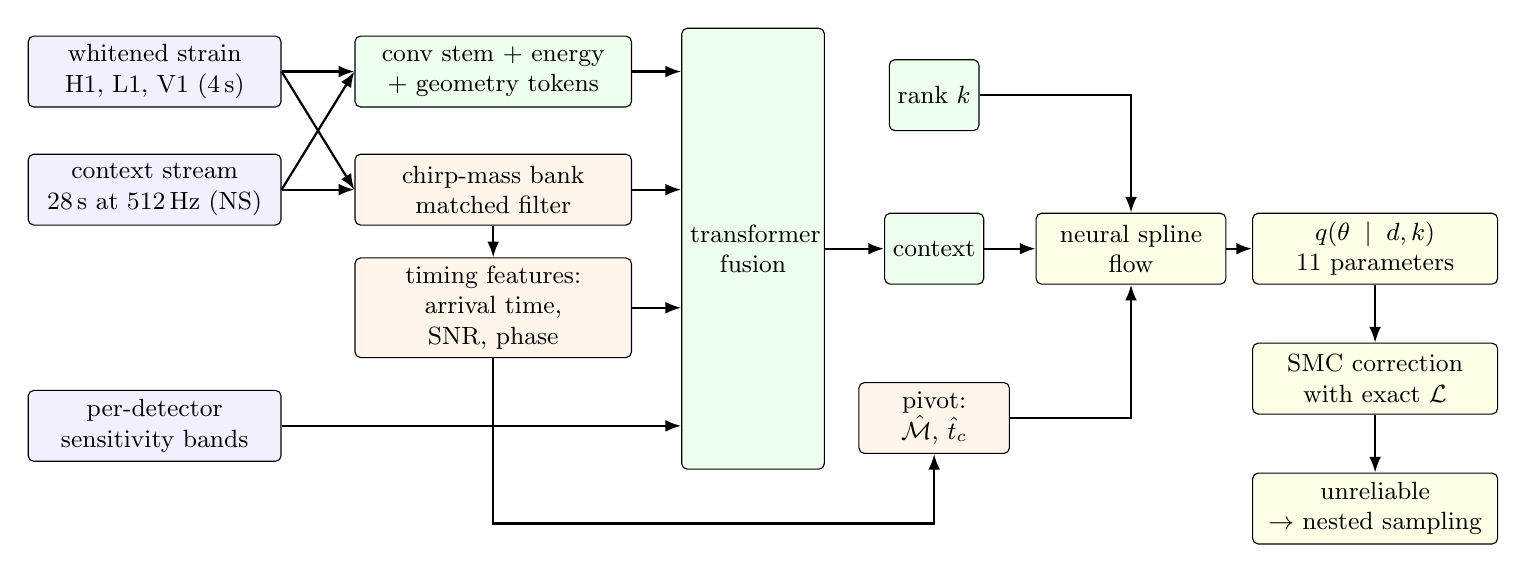
\begin{tikzpicture}[font=\small,
  box/.style={draw, rounded corners=2pt, align=center, minimum height=9mm, inner sep=3pt},
  data/.style={box, fill=blue!6, text width=3.0cm}, feat/.style={box, fill=orange!8, text width=3.3cm},
  core/.style={box, fill=green!7}, res/.style={box, fill=yellow!10, text width=2.9cm},
  arr/.style={-{Latex[length=2mm]}, thick}]
\node[data] (strain) at (0, 0)    {whitened strain\\ H1, L1, V1 (4\,s)};
\node[data] (ctx)    at (0, -1.5) {context stream\\ 28\,s at 512\,Hz (NS)};
\node[data] (asd)    at (0, -4.5) {per-detector\\ sensitivity bands};
\node[core, text width=3.3cm] (enc)  at (4.3, 0)    {conv stem + energy\\ + geometry tokens};
\node[feat] (bank) at (4.3, -1.5) {chirp-mass bank\\ matched filter};
\node[feat] (trig) at (4.3, -3.0) {timing features:\\ arrival time,\\ SNR, phase};
\node[core, minimum height=5.6cm, text width=1.6cm] (tf) at (7.6, -2.25) {transformer\\ fusion};
\node[core] (c)    at (9.9, -2.25) {context};
\node[core] (rank) at (9.9, -0.3)  {rank $k$};
\node[feat, text width=1.7cm] (piv) at (9.9, -4.4) {pivot:\\ $\hat{\mathcal M}$, $\hat t_c$};
\node[res, text width=2.2cm] (flow) at (12.4, -2.25) {neural spline\\ flow};
\node[res] (post) at (15.5, -2.25) {$q(\theta\mid d,k)$\\ 11 parameters};
\node[res] (is)   at (15.5, -3.9)  {SMC correction\\ with exact $\mathcal L$};
\node[res] (dyn)  at (15.5, -5.55) {unreliable\\ $\to$ nested sampling};
\draw[arr] (strain) -- (enc);
\draw[arr] (strain.east) -- (bank.west);
\draw[arr] (ctx.east) -- (enc.west);
\draw[arr] (ctx) -- (bank);
\draw[arr] (bank) -- (trig);
\draw[arr] (enc.east)  -- (enc.east  -| tf.west);
\draw[arr] (bank.east) -- (bank.east -| tf.west);
\draw[arr] (trig.east) -- (trig.east -| tf.west);
\draw[arr] (asd.east)  -- (asd.east  -| tf.west);
\draw[arr] (tf) -- (c);
\draw[arr] (c) -- (flow);
\draw[arr] (rank.east) -| (flow.north);
\draw[arr] (trig.south) -- ++(0,-2.1) -| (piv.south);
\draw[arr] (piv.east) -| (flow.south);
\draw[arr] (flow) -- (post);
\draw[arr] (post) -- (is);
\draw[arr] (is) -- (dyn);
\end{tikzpicture}}
\caption{LeanNPE. The encoder fuses convolutional strain tokens, inter-detector geometry tokens, chirp-mass tokens from a template-bank matched filter, and timing features from the best template; the bank's estimates $\hat{\mathcal M}, \hat t_c$ enter the flow as a pivot, and a rank embedding selects the $k$-th loudest signal. For real events the posterior is corrected against the exact likelihood; events whose replicate runs disagree are analysed with nested sampling.}\label{fig:arch}
\end{figure*}

\begin{algorithm}[t]
\algcaption{Inference for a segment with $M$ candidate signals}
\label{alg:overlap}
\begin{algorithmic}[1]
\Require whitened strain $d$, number of signals $M$
\State $c \gets \mathrm{Encoder}(d)$ \Comment{one pass, reused}
\For{$k = 0$ to $M-1$} \Comment{loudness rank}
  \State $\theta^{(1:S)}_{(k)} \sim q_\phi(\cdot \mid c, k)$ \Comment{Eq.~\ref{eq:rankposterior}}
\EndFor
\If{$M=1$} correct with Algorithm~\ref{alg:smc}
\ElsIf{$M=2$} correct jointly (Section~\ref{sec:joint})
\EndIf
\State replicate test; unreliable $\to$ nested sampling
\end{algorithmic}
\end{algorithm}

\section{Data Engine} \label{sec:training}

\subsection{Component storage and remixing}

Every simulated event is generated with \texttt{bilby} and stored as separate
whitened components -- detector noise and each individual signal -- in half
precision, rather than as one summed strain. A loader (Algorithm~\ref{alg:remix})
reassembles a different example from these components on every epoch: a fresh
noise draw, a circular time shift that moves the merger-time label with it, a
distance rescaling ($h\to s\,h$, $d_L\to d_L/s$), and for overlap examples a sum
of signals with loudness ranks re-sorted after rescaling. A fixed
signal-plus-noise sum per event lets the network memorize noise realizations:
training NLL keeps falling while validation NLL rises. Remixing removes that
channel and, by showing each signal under many noise draws, teaches the
posterior width. In the production BBH model the rescaled distance is drawn
from the training prior, so remixing does not change the prior the network
learns.

\begin{algorithm}[t]
\algcaption{Remixed batch construction}
\label{alg:remix}
\begin{algorithmic}[1]
\Require signal components $\{h_j\}$, noise pools (Gaussian, real), batch size $B$
\For{$b = 1$ to $B$}
  \State draw an event (one to four signals) and fresh noise $n$; real with probability $p_{\rm real}$
  \State if real: re-color each $h_j$ into the segment's ASD (Eq.~\ref{eq:recolor})
  \State time shift $\delta t$ (labels shifted); distance rescale $s$ ($h \gets s h$, $d_L \gets d_L/s$)
  \State drop a detector with probability $p_{\rm drop}$ (replaced by white noise)
  \State $d_b \gets \sum_j h_j + n$; sort ranks by $\mathcal{M}^{5/6}/d_L$
\EndFor
\State \Return $\{(d_b, \theta_{b,(k)}, k)\}$ for every rank $k$ present
\end{algorithmic}
\end{algorithm}

\subsection{Real detector noise} \label{sec:realnoise}

Networks trained on design-sensitivity Gaussian noise do not transfer to real
data: the spectral shape, non-stationarity and glitches of real noise differ
from the design curve in ways no amplitude rescaling repairs. We retrieve
strain segments from GWOSC \citep{Vallisneri2015Gwosc, Abbott2021Gwosc,
Abbott2023GwoscO3} -- 636 for H1, 632 for L1 and 682 for V1, spanning GPS times
from 2015 to 2025 -- whiten each with its own measured ASD $\hat S_n$, and store
strain and ASD together. Stored design-whitened signals are re-colored into
each real segment exactly,
\begin{equation}
\tilde h_{\rm real}(f) = \tilde h_{\rm design}(f)\,\sqrt{S_{n,\rm design}(f)/\hat S_{n}(f)}\;|G(f)|,
\label{eq:recolor}
\end{equation}
since whitening is diagonal in frequency. Here $G(f)$ is the response of the
15\,Hz highpass applied before $\hat S_n$ is measured, so that $\sqrt{\hat S_n}$
estimates $|G|\sqrt{S_n}$. The filter is far from flat in the band that matters
($|G|\approx0.63$ near 50\,Hz, 0.8 near 100\,Hz, unity only above about
400\,Hz), and it must be included: real strain passes through it and it cancels,
whereas stored signals do not. Omitting $|G|$ makes signals about 1.4 times too
loud in real-noise examples, a bias every simulated validation shares and so
cannot see. A network trained that way read all 34 real events too far, by a
median factor of 1.4 before the prior correction below. Injections into real noise
show it directly: with noise and source held fixed, the same network recovers
1.08 times the true distance from a signal built as in training and 1.54 times
from one passed through the real-event path, farther in 101 of 102 cases.
Certification now injects known signals through the real-event path and gates on
the amplitude ratio, right ascension and distance. The production models draw real
noise for 90\% of examples, and checkpoint selection uses the mean of the
Gaussian and real validation NLLs, so robustness in one domain cannot be bought
by losing the other. The encoder also receives a 16-band summary of each
detector's log-ASD relative to the design curve, so it knows how sensitive
each detector was.

Real-noise validation shares its noise with training in the models certified so far, BNS
and NSBH among them: the signals are held out, but the segments are drawn from the same bank,
so those real-noise coverage figures are measured on noise the network has seen.
\pending{[If the v9 model is adopted:] The final BBH model excludes every tenth segment per
observing run from training (64, 63 and 68 segments for H1, L1 and V1), and its real-noise
validation and certification use only those. The hold-out is not fully clean: that model
fine-tunes from one trained on the whole bank, so its weights carry some exposure to the
held-out segments.} The real events and the injections around them use data fetched for
each event, not the bank. One of the 1950 bank segments (L1) does contain a catalogued event,
GW190725, which is not among the events scored here.

\subsection{Datasets} \label{sec:datasets}

Each source class has its own dataset. Detector-frame masses are drawn as
follows: for BBH both components are log-uniform with $m_2\le m_1$, $p(m_1,m_2)\propto
1/[m_1 m_2\ln(m_1/m_{\min})]$, on $[5, 100]\,\msun$; for NSBH the black hole is
log-uniform on $[3, 100]\,\msun$ and the neutron star uniform on $[1, 2.5]\,\msun$;
for BNS $m_1$ is uniform on $[1, 2.5]\,\msun$ and $m_2$ uniform below it. A cap on the
primary removes low mass ratios at high chirp mass: with $m_1\le100\,\msun$ no BBH
training event at $\mathcal{M}=70$--$80\,\msun$ has $q<0.6$, although GW190706 sits
there with an LVK median of $q=0.52$. \pending{[If the v9 model is adopted:] The final
BBH dataset therefore extends $m_1$ to $200\,\msun$ under the same prior, keeping
$\mathcal{M}\le90\,\msun$, the range of the chirp-mass bank, with $1.42\times10^6$
events to keep the density of the $10^6$-event dataset below $100\,\msun$.} Aligned spins
are drawn as signed
components uniform in $[-a_{\max}, a_{\max}]$. BBH signals use IMRPhenomXP
\citep{Pratten2020PhenomXP, PrattenXPHM}; NSBH signals IMRPhenomNSBH
\citep{Thompson2020PhenomNSBH} and BNS signals IMRPhenomD\_NRTidalv2
\citep{Dietrich2019NRTidalv2}, with tidal deformabilities uniform in
$[0, 5000]$ as nuisance parameters. Signals longer than the 4\,s window are
generated on a long segment and cropped rather than wrapped, and NSBH and BNS
examples also store the whitened 28\,s before the window at 512\,Hz, where most
of their signal-to-noise ratio accumulates. Distances are drawn uniformly
within each class's detectable range (Figure~\ref{fig:distprior}): a uniform
distance prior decouples chirp mass from distance, which a $d_L^2$ prior
couples through the detection threshold; posteriors are reweighted to any
other distance prior at inference. Selection does not change this prior where
it matters. A source is kept if its stored distance lies within its horizon $T$
at the SNR threshold, and augmentation redraws distance uniformly below $T$, so
the two factors cancel and the effective prior is the assumed one cut at design
SNR $\geq 6$. Stored masses look heavier than the prior only through that cut;
weighting them by $1/(T-d_{\min})$ restores the prior (chirp-mass KS distance
0.238 to 0.015), and detected events sit far above it. Thirty percent of examples contain
overlapping signals (two to four). Table~\ref{tab:datasets} lists each dataset. The likelihood is a separate choice:
the BBH catalogue correction and \texttt{dynesty} use IMRPhenomXHM, so the correction can
use higher modes the network's training signals lack, and NSBH and BNS use their
training waveforms.

\begin{deluxetable}{lccccc}
\tablecaption{Datasets. Each stores its full generator configuration and per-shard seeds (first seed listed) in \texttt{dataset\_config.yaml}. All have a uniform distance prior, signed aligned spins, $\mathrm{SNR}\geq6$ at design sensitivity and 30\% overlapping examples, split 80/10/10 by event. \label{tab:datasets}}
\tablehead{\colhead{Class} & \colhead{Events} & \colhead{Waveform} & \colhead{$m_1$ ($\msun$)} & \colhead{$d_L$ (Gpc)} & \colhead{Seed}}
\startdata
BBH & $2\times10^5$ & IMRPhenomXP & 5--100 & 0.1--4 & 2026 \\
BBH & $10^6$ & IMRPhenomXP & 5--100 & 0.1--6 & 4096 \\
BBH (harmonics test) & $5\times10^5$ & IMRPhenomXPHM & 5--100 & 0.1--6 & 6606 \\
\pending{BBH (v9)} & \pending{$1.42\times10^6$} & \pending{IMRPhenomXP} & \pending{5--200} & \pending{0.1--6} & \pending{9009} \\
NSBH & $2\times10^5$ & IMRPhenomNSBH & 3--100 & 0.02--1.2 & 2026 \\
BNS & $2\times10^5$ & IMRPhenomD\_NRTidalv2 & 1--2.5 & 0.01--0.4 & 2026 \\
\enddata
\end{deluxetable}

\begin{figure*}[t]
\centering
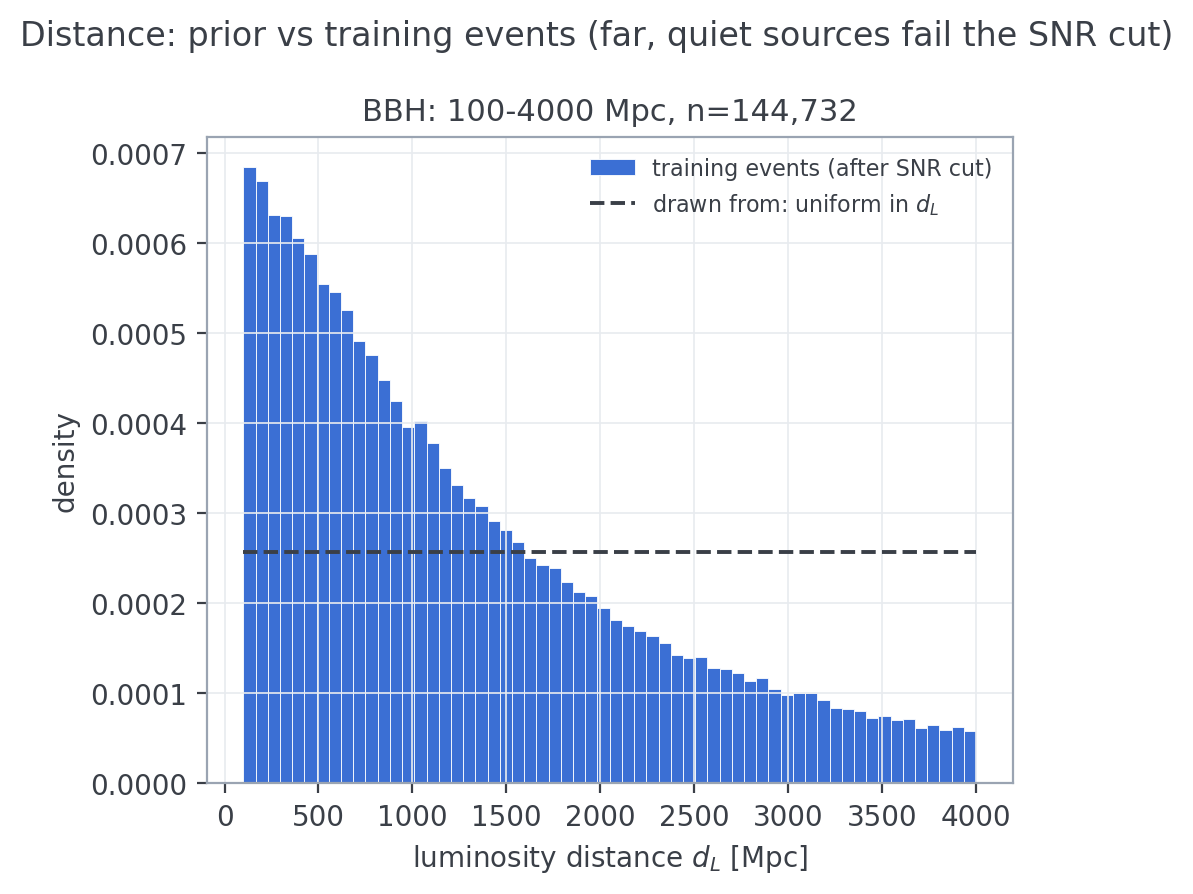
\includegraphics[width=0.32\textwidth]{distance_bbh_v4.png}\hfill
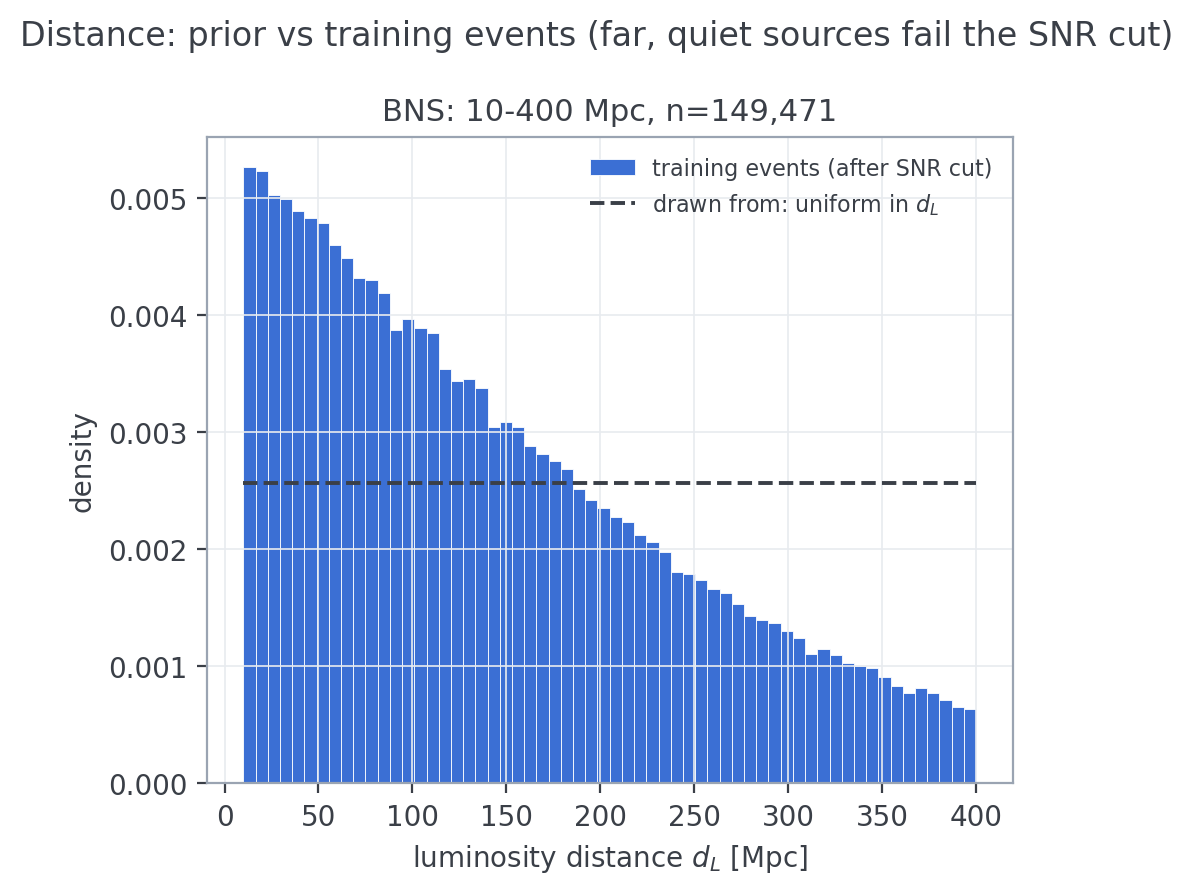
\includegraphics[width=0.32\textwidth]{distance_bns_v4.png}\hfill
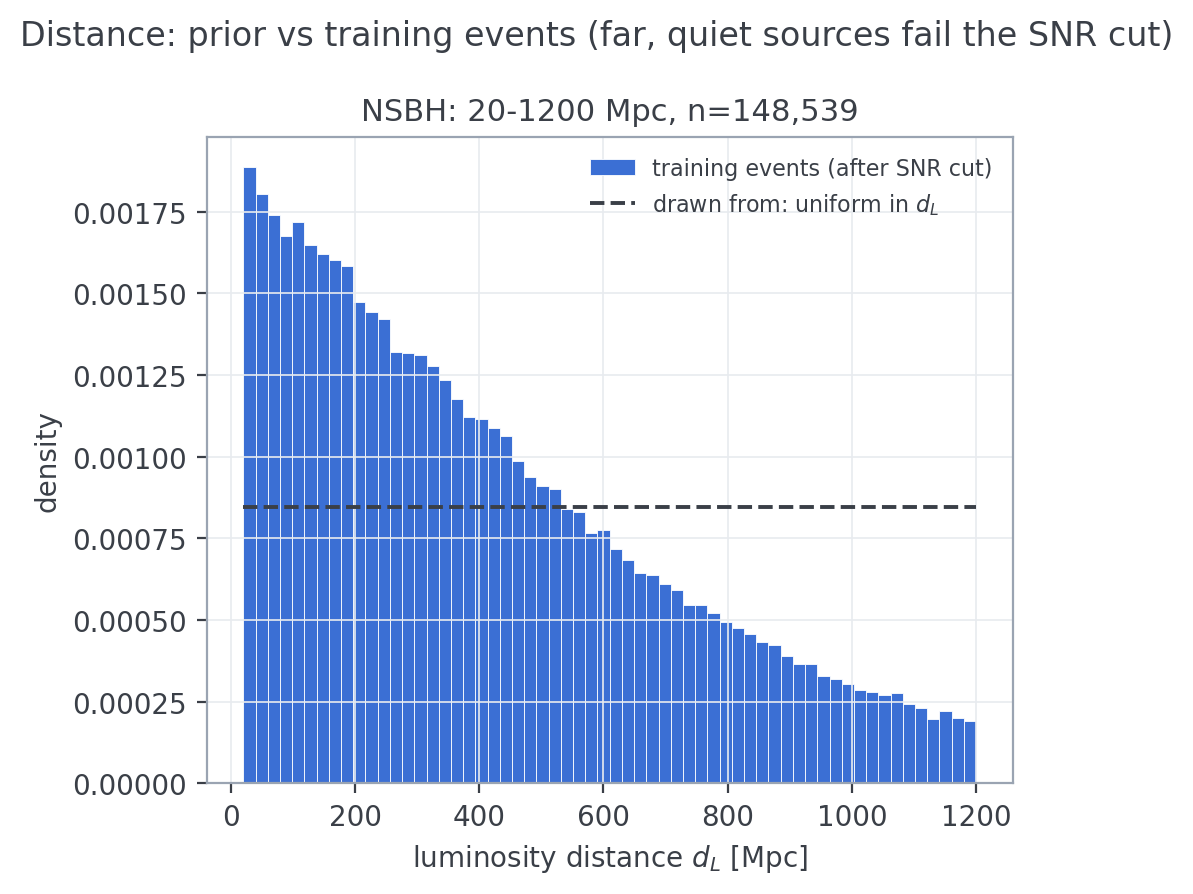
\includegraphics[width=0.32\textwidth]{distance_nsbh_v4.png}
\caption{Luminosity distance of the training events (histograms) against the uniform prior they were drawn from (dashed), for the BBH ($2\times10^5$ events), BNS and NSBH datasets. The decline at large distance is the SNR selection.}
\label{fig:distprior}
\end{figure*}

\section{Neural Posterior Estimator} \label{sec:npe}

\subsection{Strain encoder}

Whitened strain from each detector (4\,s at 4096\,Hz) passes through an
$\mathrm{asinh}$ compression and a convolutional stem with no normalization
layers into tokens; a parallel branch carries per-window log-energies of the
uncompressed strain. Because whitened noise sits at unit variance, absolute
amplitude is a distance cue, and per-sample normalization would erase it. A
geometry branch computes, per frequency band, the power-weighted complex
coherence between detector pairs (magnitude and phase) and generalized
cross-correlation arrival-time delays, and injects them as tokens. Detector
embeddings, sinusoidal positions and a three-layer pre-norm transformer
\citep{Vaswani2017Attention} ($d_{\rm model}=192$) attend jointly over all
detectors' tokens; eight learned queries pool the sequence into the context.
During training each detector is dropped with probability 0.2 and the geometry
tokens with probability 0.25, so the network neither depends on all three
detectors nor on one feature group.

\subsection{Matched-filter features}

A convolutional stem downsamples time and cannot resolve the sub-millisecond
delays that sky position depends on; a matched filter can. Each model carries
a template bank, matched-filtered in the frequency domain on the GPU
\citep{Allen2012Findchirp} for every training example. The BBH bank spaces
chirp mass by 0.5\% from 4.2 to 90\,$\msun$ and has 24 slots in mass ratio and
aligned spin (four mass ratios from 0.15 to 0.9, six spins from $-0.6$ to
0.85); the NSBH bank has signed black-hole spins; the BNS bank also filters the
28\,s context stream. The filter is evaluated coarse to fine (every chirp mass
coarsely, the neighbourhood of the best at twice the lag resolution), and
detectors must agree on the arrival time within $\pm12$\,ms. The resulting
network-SNR profile over chirp mass, and the peak chirp mass and SNR of every
slot, become \emph{chirp-mass tokens}. The best template's complex SNR series
at 0.12\,ms resolution yields \emph{timing features}: each detector's
parabolically interpolated arrival time, peak SNR and phase, pairwise delays
and phase differences, and the times and SNRs of the two strongest network
peaks, so that a second merger-time mode is visible. On simulated BBH these
recover the H1--L1 delay to 0.25\,ms at network SNR 15--25 and the merger time
to 1--2\,ms.

\subsection{Rank-conditioned neural spline flow with a pivot}

The context concatenates the pooled encoding with a learned rank embedding
($k=0,\dots,4$) and conditions a neural spline flow \citep{Durkan2019Nsf,
nflows} of ten autoregressive rational-quadratic layers with 256 hidden units
and sixteen bins, mapping a standard normal $z$ to the parameters:
\begin{equation}
\ln q_\phi(\theta \mid c) = \ln \mathcal{N}\!\big(T_\phi^{-1}(\theta;c);\,0,I\big) + \ln\Big|\det \frac{\partial T_\phi^{-1}(\theta;c)}{\partial\theta}\Big|.
\label{eq:flowdensity}
\end{equation}
Masses are parametrized as $(\ln\mathcal{M}, q)$. Parameters are mapped to
$[-1,1]$ by a fixed, deterministic scaler (logarithmic for chirp mass and
distance, linear otherwise), never by fitted statistics that could drift
between training and inference; right ascension, phase and polarization wrap
exactly at sampling. The distance support is stored in the checkpoint.
Signals are injected at one fixed epoch, so the network's right ascension is
relative to the Earth at that epoch. For an event at time $t$ we report
$\alpha + {\rm GMST}(t) - {\rm GMST}(t_{\rm ref})$, a rotation with unit Jacobian
that the correction inverts when evaluating the flow's density. On real-noise
injections through the real-event path this reduces the median right-ascension
error from 1.48 to 0.27\,rad; a tail of larger errors remains, as expected from the
sky degeneracies of events with few detectors,
and with a flat likelihood the correction still returns the prior (worst KS
distance 0.021, and 0.018 with the phase sampled explicitly).

A network that must carry a chirp mass known to $10^{-3}$ through several
layers blurs it. With the pivot, the flow instead models
$\ln\mathcal{M}-\ln\hat{\mathcal{M}}$ and $t_c-\hat t_c$, where $\hat{\mathcal
M}$ and $\hat t_c$ are the bank's estimates, passed as context and subtracted
inside the flow. A shift has unit Jacobian, so density evaluation stays exact,
and unlike a rescaling it never excludes the truth when the estimate is wrong.

\subsection{Objective}

Training minimizes Equation~\ref{eq:sbiobjective} over the remixed
distribution, with every signal rank of an example evaluated in one flow call,
plus one auxiliary term: a smooth-$L_1$ regression of the loudest signal's
scaled masses from the encoder context, weight 1. It penalizes contexts that
collapse distinct heavy, near-equal-mass systems onto one representation, a
failure the NLL alone did not prevent. The BBH model has $9.2\times10^6$
trainable parameters, $3.0\times10^6$ of them in the encoder. A forty-epoch
class model trains in four to six hours on one H100 GPU.

\section{Likelihood Correction} \label{sec:correction}

\subsection{Tempered sequential Monte Carlo}

The network's posterior is fast but approximate; on real events it is the
proposal of a sequential Monte Carlo sampler \citep{DelMoral2006Smc}
(Algorithm~\ref{alg:smc}) that evaluates the exact likelihood. Particles are
drawn from an \emph{anchor} density $a(\theta)$ built from the network's
samples and moved through the geometric bridge
\begin{equation}
\pi_\beta(\theta) \propto a(\theta)^{1-\beta}\,\big[\mathcal{L}(\theta)\,\pi(\theta)\big]^{\beta},
\label{eq:bridge}
\end{equation}
which is the anchor at $\beta=0$ and the posterior at $\beta=1$; between
stages the incremental weight is $[\mathcal{L}\pi/a]^{\beta'-\beta}$. All
densities are evaluated in the unbounded sampling coordinates, including the
Jacobian of the map. The anchor is a Gaussian mixture fitted to the network samples with
covariances inflated fourfold and with sky position and aligned spins
replaced by their prior, so that no sky island or spin branch the network
under-weights is disfavoured at intermediate temperatures. Each stage chooses
the largest $\beta$ that keeps the effective sample size at half the particle
count, resamples systematically within posterior branches (Gaussian-mixture
clusters) while keeping at least 5\% of the particles on every branch with
exact carried weights, and applies Metropolis--Hastings moves that leave the
tempered target invariant. Sampling uses unbounded coordinates (logit and
$\tanh^{-1}$ maps, wrapped angles) with exact Jacobians.

Four move types are used; each is a Metropolis--Hastings kernel that leaves
the current tempered target invariant:
\begin{enumerate}
\item random walk with the covariance of the particle's current branch, with
  the Hastings term for steps that cross branches;
\item independence proposals from the fitted mixture;
\item \emph{sky jumps}: reflection through the detector plane, rotations about
  any detector baseline, and a rotation that changes one inter-detector delay
  by $\pm12$\,ms (the cycle-slip images of a two-detector network), with
  polarization and distance redrawn by matching the detector response;
\item \emph{ridge moves}: steps in symmetric mass ratio at fixed chirp mass with
  the primary spin set to preserve the 1PN and 1.5PN phase, which follow the
  mass-ratio--spin degeneracy.
\end{enumerate}

For dominant-mode waveforms the likelihood is marginalized analytically over
phase and merger time; for higher-mode waveforms such as IMRPhenomXHM
\citep{GarciaQuiros2020XHM}, where the phase marginalization is not exact, the
phase is sampled explicitly.

Exact likelihood evaluation and invariant moves do not by themselves guarantee
that a finite run has converged, and we treat convergence as an empirical
question with three checks: a flat-likelihood test, in which the sampler must
return the prior (worst one-dimensional Kolmogorov--Smirnov distance 0.02 with
marginalized and 0.04 with sampled phase); agreement between independent
replicates on every event (Section~\ref{sec:reliability}); and agreement with
\texttt{dynesty} on the same likelihood (Sections~\ref{sec:inclination}
and~\ref{sec:overlap}). Where these disagree, as for the branch weights of
GW200115 (Section~\ref{sec:gw200115}), the event is handed to nested
sampling.

\begin{algorithm}[t]
\algcaption{Likelihood correction (one replicate)}
\label{alg:smc}
\begin{algorithmic}[1]
\Require network samples $\theta^{(1:S)}$, strain, PSDs, prior $\pi$
\State fit anchor $a$ (mixture $\times4$, flat sky and spins); draw particles from $a$
\State $\beta \gets 0$
\While{$\beta < 1$}
  \State $\beta' \gets$ largest value with ESS $\geq S/2$; reweight by $[\mathcal{L}\pi/a]^{\beta'-\beta}$ (Eq.~\ref{eq:bridge})
  \State resample within branches, each branch $\geq 5\%$
  \State move: random walk, independence, sky jumps, ridge moves
  \State $\beta \gets \beta'$
\EndWhile
\State \Return weighted particles, efficiency
\end{algorithmic}
\end{algorithm}

\subsection{Real data}

Published LVK PSDs, where available, are used in the likelihood only; the
network is still fed strain whitened with the PSD measured from the data,
since whitening its input with a different PSD moves it off its training
distribution. The likelihood segment is sized to the signal: the
leading-order chirp time from 20\,Hz of the lightest plausible chirp mass in
the network posterior, plus the time to the end of the window, rounded up to a
power of two (at least 4\,s). A fixed 16\,s segment let a long, light template
fit a transient 12\,s before GW190513, moving its chirp mass to 7.0\,$\msun$
for every seed against LVK's 29.9; with the signal-sized segment the
correction gives 31.6 [27.7, 35.7]\,$\msun$. Detectors whose whitened strain
contains excursions beyond any training signal ($50\sigma$) are replaced by
white noise, as an absent detector is in training; a detector is kept when
the data around the trigger are valid even if the fetched span has gaps
elsewhere. The one exception is a short glitch with a known time, which is gated instead.
GW170817's L1 glitch reaches $137\sigma$ about 1\,s before the merger, and dropping the
most sensitive detector costs almost all sky information: against the optical position
\citep{Abbott2017GW170817} the network alone gives a right ascension error of 2.37\,rad over about
17000\,deg$^2$ without L1, and 0.10\,rad over about 1150\,deg$^2$ with a gate, zero within
0.2\,s of the glitch and tapered over a further 0.1\,s, applied above 10\,Hz so the cut
leaks no low-frequency power. The network never trained on such gaps. Twenty injections at
network SNR 15 with a matching gap give 0.43\,rad, against 0.27\,rad with the data
intact and 1.09\,rad without L1, with mean searched fractions of 0.45--0.58, consistent with 0.5 at this sample size (standard error 0.065). Network and likelihood read the
same gated strain, and the result carries a warning.

Every likelihood stops at 1700\,Hz. GWOSC 4\,kHz strain is low-passed, and above that
frequency its ASD falls to 1--3\% of the 300\,Hz level. A real signal passes through the
filter with the noise, but a template does not, so dividing it by that ASD inflates it. With
the limit at Nyquist the optimal SNR is 1.16--1.30 times too high for a BNS and 1.15--1.28
for a 6+1.4\,$\msun$ NSBH, and unchanged for an 8.9+1.9\,$\msun$ NSBH and for BBH down to
8+5\,$\msun$, whose signals end below the limit. Training data are not affected: after
re-coloring, a median of 0.3\% of BNS power lies above 1700\,Hz.

\subsection{Reliability} \label{sec:reliability}

Each event is corrected twice with different seeds and the particles are
pooled. The result is marked unreliable, and handed to nested sampling, when
the replicate medians differ by more than one 90\% width or the corrected
chirp mass falls outside the network's 99\% support. Multimodal posteriors are
where this matters: importance-based methods find every mode but can misweight
them (Section~\ref{sec:gw200115}).

\subsection{Two overlapping signals} \label{sec:joint}

For two signals the correction samples the 22-parameter joint posterior with
the likelihood of the summed waveforms (Equation~\ref{eq:jointlikelihood}),
starting from the network's rank-0 and rank-1 answers and keeping the
training's loudness ordering, so the labels do not switch. Two additional
moves make this tractable: each signal's merger time and phase are drawn from
their exact tempered conditional (one FFT over all time shifts and a von Mises
draw), which escapes the cycle-spaced local maxima of the joint likelihood;
and block moves redraw one signal from a mixture of refined and raw network
samples and prior draws, with the reverse proposal densities in the
acceptance ratio. The proposal is refined
by alternating single-signal corrections on residuals with the best-fit
waveform of the other signal subtracted.

\section{Data-Quality Indicators} \label{sec:ood}

Every posterior carries diagnostics: the fraction of samples railing at the
edge of the scaled support, a Mahalanobis distance of the context to the
training contexts with its validation percentile, data-quality heuristics on
the strain (whitened standard deviation, peak amplitude, excess kurtosis), and
for corrected posteriors the replicate spread and sampling efficiency. They
combine into a \texttt{HIGH}/\texttt{MEDIUM}/\texttt{LOW} label. These are indicators of
how unusual an event is, not calibrated probabilities: we have not measured the failure
rate within each label, and a \texttt{HIGH} label does not guarantee a correct posterior.
GW190814, whose secondary lies above the NSBH network's 2.5\,$\msun$ limit, receives
\texttt{HIGH} while the LVK mass ratio falls outside its 90\% interval. The
likelihood correction's replicate test is the only diagnostic that acts
automatically.

\section{Experimental Setup} \label{sec:setup}

\paragraph{Certification.} Every checkpoint runs a fixed suite on 2000
held-out events in Gaussian and 2000 in real noise: coverage at 50/68/90/95\%,
SBC for all parameters, the shuffle statistic, railing, distance correlation
and per-class distance bias, the growth of chirp-mass width with SNR,
permutation importance of feature groups, six GWTC smoke tests, and a matched
comparison with \texttt{dynesty}: 30 simulated BBH events, stratified in SNR
from 8 to 60 and drawn from the training prior, analysed once by
\texttt{dynesty} and stored, so every checkpoint is judged on exactly the same
strains.

Two gates compare the training and real-event paths directly. Re-coloring makes the same
validation events quieter (median SNR 13.6 in Gaussian noise, 8.1 in real noise), and NLL depends
strongly on SNR, so the raw difference between the two NLLs mostly measures loudness. We
therefore bound the difference by less than 3\,nats within the SNR bins 10--20 and
20--40, where real events sit, with each domain binned by its own SNR. These are comparisons
of populations, not of paired events. The second gate injects known signals into data
around real events, through the real-event path, at network SNR 15: 36 for BBH and 40 each for NSBH and
BNS. BBH injections go 20\,s before the event; NSBH and BNS go 32\,s after, so that their 28\,s context stream is
clear of the event and its glitch, and they carry the inspiral through that stream.
Injections are low-passed like the data above 1700\,Hz. Without that, 54--70\% of a BNS
injection's whitened power fell above 1900\,Hz, so ``SNR 15'' was really quieter. The gate requires the amplitude ratio between
the paths within 0.90--1.15, the median posterior distance within 0.75--1.25 of the truth, and the median error of the mean
right ascension below 0.5\,rad over injections with a second detector at SNR $\geq 5$, of
which there must be at least four. The mean searched fraction of the true sky position
over all injections must lie within $0.5\pm0.2$; the density and the mass are taken from
separate halves of the samples, since reading both off one histogram biases it high
(0.60 for a calibrated uniform sky). We set the SNR binning and the sky selection after seeing
models fail the earlier versions of these gates, for reasons the audits above identified, and report them
as such. The thresholds themselves did not change. The distance median is weighted by each injection's true distance. Angles are isotropic at fixed SNR, and
under a uniform distance prior such events occur in proportion to their distance, so an ideal posterior reads about 1.19 times the truth unweighted (0.74--1.85 between the 10th and 90th percentiles) and 1.00 weighted. Unweighted, the BNS and NSBH medians were 1.17--1.18 over eight injection seeds, ranging from 0.87 to 1.43 per seed.

\paragraph{Real events against LVK, alongside DINGO.} We analysed 34 O3 BBH
events with the full pipeline (network, correction with IMRPhenomXHM, the
PSDs of the LVK analyses, two replicates, 46 CPU cores), and ran DINGO
\citep{Dax2021Dingo, Dax2023DingoBns} with its released O3 networks and
importance sampling on the same events, given the same LVK PSDs and the LVK
distance prior (uniform in source frame to 6\,Gpc). 28 events have results from
both: DINGO produced none for three (GW190620, GW190910, GW200302), and our run
has none for three events observed without H1 (GW190630, GW190708,
GW200112), for which the data retrieval required a detector the LVK analysis
did not use; these are being rerun. Every posterior is reweighted to the LVK
priors, including a distance prior uniform in comoving volume as in the
released cosmological LVK samples and the DINGO runs, and judged against the published LVK posterior of the same event:
offset of the median in LVK standard deviations, 90\% width relative to LVK's,
and whether the LVK median lies inside the 90\% interval.

\paragraph{Reference sampler.} \texttt{dynesty} is a reference, not ground truth, so
we also check it. It uses 1000 live points unless stated; \pending{selected real events are
repeated with independent seeds and with 2000 live points, and we report the spread in the
evidence and in the posterior medians and widths [numbers pending].}

\paragraph{Overlap capacity.} Events with $k=1,\dots,6$ signals are built by
summing $k$ independent held-out signals and one noise draw, the composition
the training remix uses, and every rank the network has is queried (300 events
per $k$).

\section{Results} \label{sec:results}

\subsection{Calibration} \label{sec:calibration}

\begin{deluxetable}{lcccc}
\tablecaption{Certification of the BBH network ($10^6$-event dataset, 30 epochs) on 2000 held-out events per noise domain. Coverage is at the 90\% level. \label{tab:cert}}
\tablehead{\colhead{Parameter} & \colhead{Cov$_{90}$ Gauss.} & \colhead{Cov$_{90}$ real} & \colhead{SBC $p$ G.} & \colhead{SBC $p$ real}}
\startdata
mass\_1 & 0.897 & 0.899 & 0.085 & 0.095 \\
mass\_2 & 0.900 & 0.894 & 0.005 & 0.161 \\
luminosity\_distance & 0.900 & 0.899 & 0.259 & 0.146 \\
ra & 0.893 & 0.885 & 0.679 & 0.789 \\
dec & 0.899 & 0.892 & 0.146 & 0.365 \\
theta\_jn & 0.893 & 0.890 & 0.178 & 0.530 \\
psi & 0.909 & 0.906 & 0.161 & 0.259 \\
phase & 0.911 & 0.910 & 0.029 & 0.054 \\
geocent\_time & 0.890 & 0.892 & 0.604 & 0.009 \\
a1 & 0.894 & 0.902 & 0.095 & 0.047 \\
a2 & 0.891 & 0.895 & 0.460 & 0.060 \\
\enddata
\end{deluxetable}

The BBH network has near-nominal marginal coverage in every parameter and both
noise domains (Table~\ref{tab:cert}): 90\% coverage lies between 0.885 and 0.911, and
the 50\% coverage between 0.48 and 0.52 on Gaussian noise. With 2000 events each 90\%
coverage carries a binomial standard error of 0.0067, or $\pm0.013$ at 95\% confidence,
so the extremes are small but not all within sampling noise. SBC passes our threshold ($p>10^{-3}$)
for all eleven parameters in both domains, but that threshold is permissive: four of
the 22 values lie below 0.05, where about one is expected by chance, so some rank
non-uniformity remains (mass\_2 and phase in Gaussian noise, geocent\_time and a1 in real noise). Marginal coverage and marginal SBC
do not test parameter correlations or the far tails. No post-hoc recalibration is applied. The posterior depends strongly on
the data: the shuffle statistic is 30.4\,nats in Gaussian and 24.8\,nats in
real noise. Distance is unbiased (median true/predicted 0.98) with a
correlation of 0.91 (real noise: 0.88) between posterior median and truth, and
0.3\% of samples rail. Figure~\ref{fig:v5coverage} shows 90\% coverage in real
noise for all three class models, 0.875--0.905 throughout.

\begin{figure*}[t]
\centering
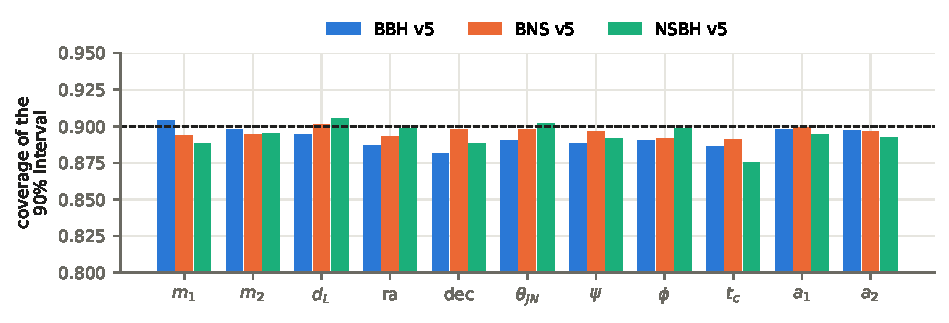
\includegraphics[width=0.9\textwidth]{coverage_real.pdf}
\caption{Coverage of the 90\% credible interval in real O3 noise, 2000 held-out events per class model ($2\times10^5$-event BBH model). The dashed line is the nominal 0.9.}
\label{fig:v5coverage}
\end{figure*}

\subsection{Precision against \texttt{dynesty}} \label{sec:matched}

On the 30 matched injections the BBH network's 90\% chirp-mass interval is
1.03 times as wide as \texttt{dynesty}'s in the median, and its mass-ratio
interval 1.10 times; the truth lies in the network's 90\% chirp-mass interval
for 93\% of events and in its mass-ratio interval for all of them. The ratio
depends on loudness: 0.7 at SNR 8--20, 1.4 at 20--35 and 2.1 above 35
(Figure~\ref{fig:v5dynesty} shows the same comparison for the
$2\times10^5$-event model, 1.36 overall). An estimator limited only by the
data has posterior width $\propto1/\mathrm{SNR}$, so width times SNR is flat;
the network's grows from 1.9 to 3.9 (scaled units) between SNR 10 and the
loudest bin. Above SNR 35 the network therefore leaves information in the
data, and the likelihood correction recovers it. Section~\ref{sec:experiments}
investigates why.

\begin{figure}[htbp]
\centering
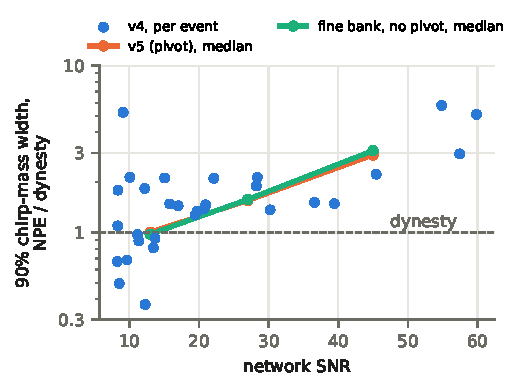
\includegraphics[width=\columnwidth]{dynesty_width_ratio.pdf}
\caption{Ratio of 90\% chirp-mass widths, network over \texttt{dynesty}, on identical simulated BBH strain, against network SNR ($2\times10^5$-event BBH model, with and without the pivot).}
\label{fig:v5dynesty}
\end{figure}

\subsection{What the network uses}

Shuffling one feature group across the events of a batch and measuring the
rise in validation NLL shows which inputs the trained network reads
(Figure~\ref{fig:v5importance}). The chirp-mass bank and timing tokens
account for 14.8 and 14.3 of the 23.4\,nats lost when the whole BBH input is
shuffled; shuffling the timing tokens multiplies the merger-time error by about
one hundred and the right-ascension error by fifteen. On BNS, where the
timing features matter most, eight-epoch runs that differ only in these
features (Figure~\ref{fig:v5timing}) move right ascension and declination from
the prior (posterior width 0.94 and 1.02 of the prior's) to 0.43 and 0.80,
halve the merger-time width, improve the validation NLL by 2.8\,nats per
event, and bring both BNS certification events, GW170817 and GW190425
\citep{Abbott2017GW170817, Abbott2020GW190425}, from 1.3\,s off their triggers
to within 0.04\,s.

\begin{figure}[htbp]
\centering
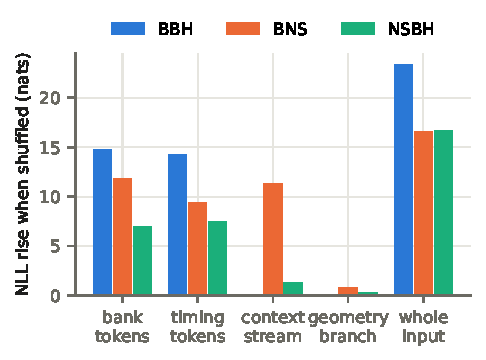
\includegraphics[width=\columnwidth]{feature_importance.pdf}
\caption{Permutation importance: rise in validation NLL per event when one feature group is shuffled across events, for the three class models.}
\label{fig:v5importance}
\end{figure}

\begin{figure}[htbp]
\centering
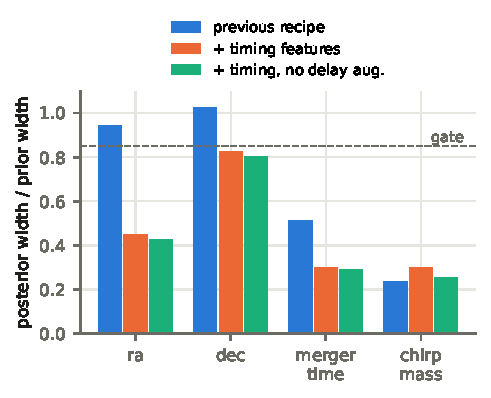
\includegraphics[width=\columnwidth]{timing_ab.pdf}
\caption{Matched-filter timing features on BNS (eight epochs, otherwise identical runs): posterior width relative to the prior for sky position, merger time and chirp mass; 1 means unmeasured. The dashed line marks the certification threshold.}
\label{fig:v5timing}
\end{figure}

The pivot is the largest single gain for neutron-star systems: it improves the
BNS validation NLL from $-10.74$ to $-13.55$\,nats per event and flattens the
growth of chirp-mass width times SNR from a factor 1.82 to 1.32
(Table~\ref{tab:classes}).

\begin{deluxetable}{lcccl}
\tablecaption{Class models: validation NLL per event in Gaussian and real noise, chirp-mass posterior width relative to the prior, and certification. \label{tab:classes}}
\tablehead{\colhead{Model} & \colhead{NLL$_{\rm G}$} & \colhead{NLL$_{\rm real}$} & \colhead{$\mathcal{M}$ width} & \colhead{Gates}}
\startdata
BBH, no pivot ($2\times10^5$) & $-7.38$ & $-4.71$ & 0.29 & one fails$^a$ \\
BBH, pivot ($2\times10^5$) & $-10.14$ & $-6.66$ & 0.28 & two fail$^b$ \\
BBH, pivot ($10^6$, 6\,Gpc) & $-12.65$ & $-8.53$ & 0.24 & two fail$^b$ \\
BNS, no pivot & $-10.74$ & $-9.33$ & 0.43 & all pass \\
BNS, pivot & $-13.55$ & $-11.71$ & 0.41 & all pass \\
NSBH, no pivot & $-9.48$ & $-8.00$ & 0.49 & all pass \\
NSBH, pivot & $-10.56$ & $-8.87$ & 0.45 & one fails \\
\enddata
\tablecomments{$^a$A fixed-reference \texttt{dynesty} gate later replaced by the matched comparison. $^b$Growth of chirp-mass width times SNR (ratio 2.03 against 2.0 for the $10^6$ model), and the Gaussian--real NLL gap (4.1 against 3\,nats). The NSBH model in use omits the pivot (Section~\ref{sec:gw200115}).}
\end{deluxetable}

\subsection{Inclination and distance on matched injections} \label{sec:inclination}

The network's own inclination posterior is close to the prior, and because
distance and inclination are degenerate in the signal amplitude, distance
suffers with it. Figure~\ref{fig:inclination} compares three methods on
identical strain: six GW150914-like injections at network SNR 25 in design
noise, at $\theta_{JN} = 0.3$, 0.9 and $\pi/2$ and two sky positions. For the
inclined and face-on systems all three methods are broad, since near face-on the
polarization ratio $2\cos\theta_{JN}/(1+\cos^2\theta_{JN})$ changes only to
second order; the correction matches \texttt{dynesty}'s 90\% interval of
$|\cos\theta_{JN}|$ to within 0.05. For the edge-on systems \texttt{dynesty}
confines $|\cos\theta_{JN}|$ to $[0.00, 0.03]$ and $[0.00, 0.08]$, the network
spans $[0.01, 0.91]$ and $[0.03, 0.93]$, and the correction gives $[0.00,
0.03]$ and $[0.00, 0.08]$. Distance follows: for the edge-on system at
431\,Mpc the network's median is 761\,Mpc, the corrected medians 385--398\,Mpc
over four seeds, and \texttt{dynesty}'s 409\,Mpc. This injection has three sky
islands; \texttt{dynesty} (500 and $2\times1500$ live points) puts less than
0.4\% of its posterior on the mirror island that contains the truth, while
importance sampling of each island under the same likelihood and prior gives
about 4\%, as does the correction, whose moves equilibrate to the same value
when started from \texttt{dynesty}'s posterior.

\begin{figure*}[t]\centering
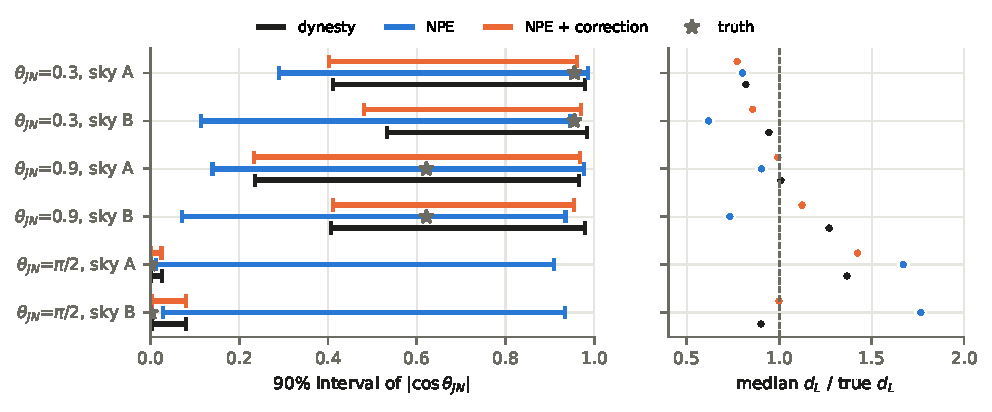
\includegraphics[width=\textwidth]{figures/inclination_is.pdf}
\caption{Inclination and distance on matched injections (GW150914-like, network SNR 25, design noise; identical strain for every method). Left: 90\% intervals of $|\cos\theta_{JN}|$ for \texttt{dynesty}, the network alone, and the corrected posterior; stars mark the truth. Right: posterior median distance relative to the truth.}
\label{fig:inclination}
\end{figure*}

\subsection{Real events against the LVK posteriors} \label{sec:dingo}

\begin{deluxetable*}{lcccccc}
\tablecaption{28 O3 BBH events analysed by both systems with the same LVK PSDs, judged against the LVK posteriors (medians over events). $|\Delta|$: offset of the median from the LVK median in LVK posterior standard deviations; $w_{90}$: 90\% width relative to LVK's; in$_{90}$: fraction of events whose LVK median lies inside the method's 90\% interval. \label{tab:dingo}}
\tablehead{\colhead{Method} & \multicolumn{2}{c}{chirp mass} & \multicolumn{2}{c}{mass ratio} & \multicolumn{2}{c}{distance} \\ \colhead{} & \colhead{$|\Delta|$ ($w_{90}$)} & \colhead{in$_{90}$} & \colhead{$|\Delta|$ ($w_{90}$)} & \colhead{in$_{90}$} & \colhead{$|\Delta|$ ($w_{90}$)} & \colhead{in$_{90}$}}
\startdata
\pending{LeanNPE network} & \pending{0.75 (1.24)} & \pending{93\%} & \pending{0.40 (1.19)} & \pending{100\%} & \pending{1.28 (1.27)} & \pending{89\%} \\
\pending{LeanNPE corrected} & \pending{0.17 (0.98)} & \pending{100\%} & \pending{0.17 (0.99)} & \pending{100\%} & \pending{\textbf{0.36} (1.00)} & \pending{96\%} \\
DINGO network & 0.30 (1.21) & 96\% & 0.20 (1.03) & 100\% & 0.51 (1.19) & 100\% \\
DINGO-IS & \textbf{0.15} (0.99) & 100\% & \textbf{0.14} (0.96) & 96\% & 0.48 (1.05) & 100\% \\
\enddata
\tablecomments{\pending{LeanNPE rows predate the 2026-11-05 fixes; figures \ref{fig:dingo} and \ref{fig:dingoevents} likewise.} LeanNPE rows use the $2\times10^5$-event BBH network. Six of the 34 events lack a result from one of the two systems (Section~\ref{sec:setup}).}
\end{deluxetable*}

Table~\ref{tab:dingo} and Figure~\ref{fig:dingo} summarize the comparison.
The likelihood correction is what turns LeanNPE's broad network posterior into
an LVK-like one: offsets fall from \pending{0.75, 0.40 and 1.28} to \pending{0.17, 0.17 and 0.36}
LVK standard deviations in chirp mass, mass ratio and distance, and the widths
from \pending{1.19--1.27} to \pending{0.98--1.00} of LVK's, while the LVK median stays inside the
90\% interval for 96--100\% of events. The corrected posteriors and DINGO-IS
are comparable: DINGO-IS is slightly closer to LVK in the masses (0.15 and
0.14), LeanNPE in distance (\pending{0.36} against 0.48), and event by event
(Figure~\ref{fig:dingoevents}) the corrected LeanNPE posterior is the closer of
the two on \pending{11, 10 and 15} of the 28 events in chirp mass, mass ratio and
distance. With the same median offsets of a few tenths of an LVK standard
deviation, the residual differences between either method and LVK are of the
size expected from differences in waveform model, priors and data
conditioning rather than from sampling failures. Every one of the 31 events we
completed passed the replicate test. The correction took a median of 574\,s per
event, both replicates included, on 46 CPU cores; DINGO took a median of
1064\,s to sample and 937\,s to importance-sample per event, with a sample
efficiency of 5.6\%.

Network against network, DINGO is ahead: its offsets are 0.30, 0.20 and 0.51
against our \pending{0.75, 0.40 and 1.28}, and its intervals are narrower (1.03--1.21
against \pending{1.19--1.27} of LVK's width). \pending{[Rewrite after the retrain: the
``broad rather than wrong'' reading below predates the amplitude and prior fixes,
which showed a systematic far bias in distance.]} Both networks are honest -- the LVK median
lies inside their 90\% intervals for \pending{89--100\%} of events -- so ours is broad
rather than wrong, and the correction removes the difference. DINGO's networks
are an order of magnitude larger and use GNPE's iterative time alignment;
Section~\ref{sec:experiments} tests the analogous changes for LeanNPE.

\begin{figure}[htbp]
\centering
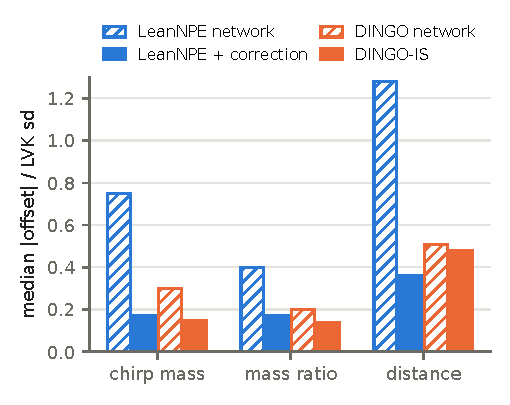
\includegraphics[width=\columnwidth]{dingo_h2h.pdf}
\caption{Median offset from the LVK posterior median, in LVK standard deviations, on the 28 O3 BBH events of Table~\ref{tab:dingo}. Hatched: network alone; solid: after likelihood correction (LeanNPE) or importance sampling (DINGO-IS).}
\label{fig:dingo}
\end{figure}

\begin{figure*}[t]
\centering
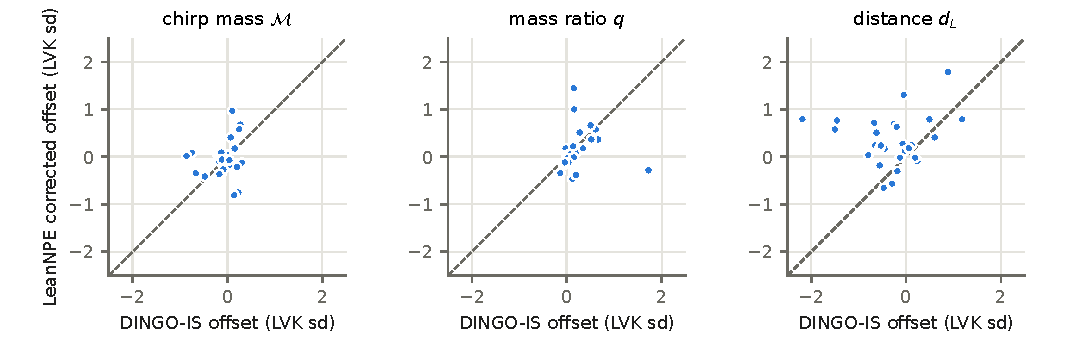
\includegraphics[width=\textwidth]{dingo_per_event.pdf}
\caption{Per-event signed offsets from the LVK median, in LVK standard deviations: corrected LeanNPE against DINGO-IS. Points on the dashed line agree; points nearer the horizontal axis favour LeanNPE.}
\label{fig:dingoevents}
\end{figure*}

\subsection{A multimodal event: GW200115} \label{sec:gw200115}

GW200115 \citep{Abbott2021NSBH} shows why the replicate test is needed. Under
our signed, uniform spin prior, \texttt{dynesty} with 1500 live points
concentrates the posterior on light black holes with strongly anti-aligned
spin, $m_1 = 4.3^{+1.4}_{-0.6}\,M_\odot$ and $a_1 \approx -0.67$, along one
curved ridge in mass and spin; the LVK analysis, with an isotropic spin prior,
reports $m_1 \approx 6.3\,M_\odot$ in the detector frame. Scoring each method by
the posterior mass it places in the four mixture components of
\texttt{dynesty}'s posterior (Figure~\ref{fig:gw200115}), the network alone puts
most of its mass at the heavy end of the ridge. A signed-spin bank with
bank-seeded initial particles recovers every part of the ridge (mode recall
0.75--1.0 against 0.25), with hundreds to thousands of particles in each, but
not \texttt{dynesty}'s weights, and replicates disagree; the event is routed to
nested sampling. The pivot sharpens unimodal posteriors but recovered this
ridge less well, which is why the NSBH model in use omits it.

\begin{figure}[htbp]
\centering
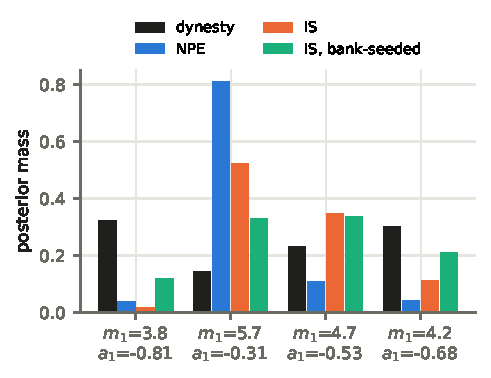
\includegraphics[width=\columnwidth]{gw200115_modes.pdf}
\caption{GW200115: posterior mass in the four mixture components of \texttt{dynesty}'s posterior (labelled by their centres), for \texttt{dynesty}, the network, and the correction without and with bank seeding.}
\label{fig:gw200115}
\end{figure}

\subsection{Overlapping signals} \label{sec:overlap}

\begin{deluxetable}{ccccc}
\tablecaption{Overlap capacity of the BBH network ($2\times10^5$ events): mean 90\% coverage over the headline parameters, and median fractional chirp-mass error, for the loudest and the quietest signal of segments with $k$ signals (300 segments per $k$; binomial 95\% uncertainty of a single coverage value $\approx\pm0.03$). Training segments hold one to four signals. \label{tab:overlap}}
\tablehead{\colhead{$k$} & \colhead{loudest: Cov$_{90}$} & \colhead{loudest: $|\Delta\mathcal{M}|/\mathcal{M}$} & \colhead{quietest: Cov$_{90}$} & \colhead{quietest: $|\Delta\mathcal{M}|/\mathcal{M}$}}
\startdata
1 & 0.91 & 2.4\% & -- & -- \\
2 & 0.84 & 4.1\% & 0.92 & 37\% \\
3 & 0.84 & 3.9\% & 0.91 & 40\% \\
4 & 0.84 & 4.8\% & 0.86 & 47\% \\
5 & 0.85 & 6.9\% & 0.73 & 41\% \\
\enddata
\end{deluxetable}

Table~\ref{tab:overlap} and Figure~\ref{fig:overlap} show how the network
handles $k$ simultaneous signals. With 300 segments per $k$, a single
parameter's 90\% coverage carries a binomial 95\% uncertainty of about
$\pm0.03$. Up to the four signals present in training, the rank-conditioned
network maintains approximately nominal marginal coverage: 0.84--0.92 across
ranks, with the louder ranks at the low end, slightly overconfident. The quieter signals
(median SNR 8--15) have broad chirp-mass posteriors (37--47\% error), as their
SNR implies, and the loudest signal's chirp-mass error grows from 2.4\% alone to
4.8\% with three companions. At $k=5$ the fifth rank, never trained, falls to
0.73 coverage, and segments with more signals than the rank embedding has
entries cannot be queried at all. The loudest signal's coverage drops from
0.91 to 0.84 as soon as a second signal is present, a mild overconfidence,
outside the binomial uncertainty, that the joint correction is designed to
remove; that correction has been validated against \texttt{dynesty} for two
signals only.

\begin{figure*}[t]
\centering
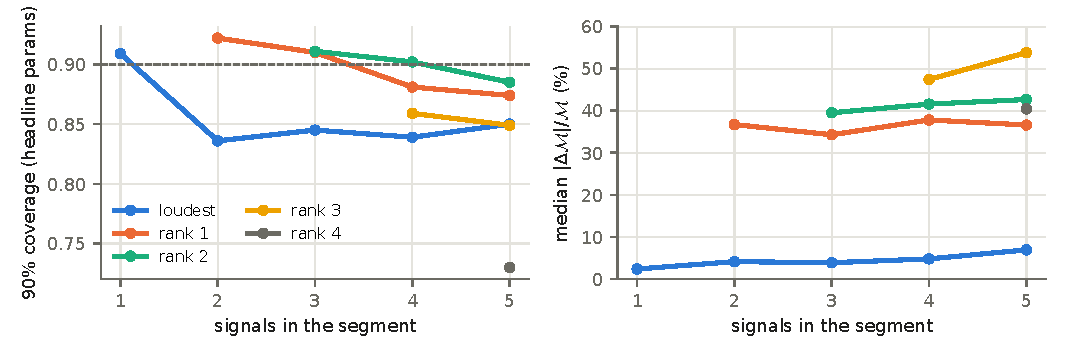
\includegraphics[width=\textwidth]{overlap_capacity.pdf}
\caption{Overlap capacity: 90\% coverage of the headline parameters (left) and median fractional chirp-mass error (right) for each signal rank, against the number of signals in the segment. Rank 4 at $k=5$ is beyond the training data.}
\label{fig:overlap}
\end{figure*}

The joint correction (Section~\ref{sec:joint}) was validated against joint
\texttt{dynesty} runs of the same 22-parameter likelihood. For an SNR-20 and an
SNR-10 signal 0.12\,s apart, the 90\% intervals of the two methods overlap by
87--100\% on all 14 headline parameters, after 22 minutes. For two SNR-20
signals the overlap is 67--100\% and the median log-likelihood ratio 358
against 361 at the truth, after 27 minutes. \texttt{dynesty} took hours on
both.

\section{Architecture Experiments for Loud Signals} \label{sec:experiments}

The network's one clear weakness is chirp-mass precision above SNR 35
(Section~\ref{sec:matched}). The certification's diagnostics place it in the
encoder rather than the flow: the ratio of posterior width to the residual of
a linear probe from context to truth is 0.64--0.75 in every run we certified,
so a larger flow cannot help. We tested six changes to the encoder and the objective, each
an eight-epoch run on the $2\times10^5$-event BBH dataset that differs from a
common baseline in that change alone (Table~\ref{tab:ab},
Figure~\ref{fig:snrscaling}).

\begin{deluxetable}{lccc}
\tablecaption{Eight-epoch architecture experiments (BBH, $2\times10^5$ events). Growth: chirp-mass width times SNR in the loudest SNR bin over the quietest (data-limited: 1). Gap: Gaussian minus real validation NLL (gate: $<3$\,nats). \label{tab:ab}}
\tablehead{\colhead{Change} & \colhead{Growth} & \colhead{Loudest bin} & \colhead{Gap}}
\startdata
baseline (24-slot bank) & 3.13 & 7.8 & 3.06 \\
120-slot bank (10 $q$ $\times$ 12 spins) & \textbf{2.40} & \textbf{6.0} & 3.07 \\
120-slot bank + trigger alignment & 2.60 & 6.7 & 2.93 \\
trigger alignment & 3.12 & 8.4 & 2.92 \\
aligned waveform-basis branch & 3.35 & 8.7 & 3.14 \\
SNR-weighted objective & 2.77 & 6.9 & 2.96 \\
low-$q$-extended bank & 3.23 & 7.8 & 2.90 \\
encoder twice as wide & 3.16 & 7.8 & 3.20 \\
\enddata
\end{deluxetable}

\paragraph{Denser bank.} Replacing the bank's 24 mass-ratio--spin slots with
120 (ten mass ratios from 0.08 to 0.95, twelve aligned spins from $-0.75$ to
0.9) narrows the loudest bin by 23\% and is the only change that moves the
growth substantially, at 4.4 times the per-epoch cost and a 7\,GB bank.

\paragraph{Trigger alignment.} GNPE's central idea, adapted: each detector's
strain is shifted by its arrival time from the bank trigger before the
convolutional stem, so the merger always sits at the same position. It
narrows the Gaussian--real NLL gap slightly (3.06 to 2.92\,nats) but does not
improve chirp-mass precision, alone or combined with the dense bank.

\paragraph{Aligned waveform-basis branch.} A branch that projects the
trigger-aligned whitened strain linearly onto the leading singular vectors of
aligned templates, preserving the phase coherence a compressing stem might
lose. It did not help.

\paragraph{SNR-weighted objective.} Weighting each event's NLL by its
matched-filter SNR, a function of the data alone, leaves the optimal posterior
unchanged (the minimizer of $\mathbb{E}_d[w(d)\,\dkl]$ is still the posterior
wherever $w>0$) and shifts capacity toward loud events. It narrows the loudest
bin by 12\% at the cost of 0.5\,nats of Gaussian NLL.

\paragraph{Capacity.} An encoder twice as wide changes nothing in eight epochs,
and a full thirty-epoch run of the wide encoder on the $10^6$-event dataset
ends 0.2--0.3\,nats per event worse in validation NLL than the standard one
in both noise domains.
Training length, by contrast, matters: the standard architecture trained for
thirty epochs on five times the data reaches a growth of 2.03.

\begin{figure}[htbp]
\centering
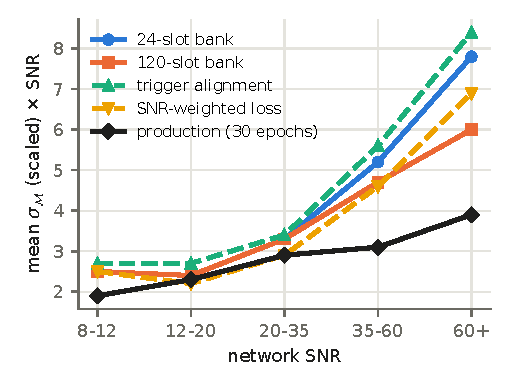
\includegraphics[width=\columnwidth]{snr_scaling.pdf}
\caption{Chirp-mass posterior width times SNR against network SNR (flat = limited only by the data). Coloured: eight-epoch runs that differ from the 24-slot baseline in one change; black: the standard architecture after thirty epochs on $10^6$ events.}
\label{fig:snrscaling}
\end{figure}

\paragraph{Where the floor is.} Since only the bank moved the growth, we probed
the bank directly, without the network: on 3000 held-out signals we computed
the chirp-mass estimate of the best slot's interpolated SNR peak, and the
estimate of the slot nearest the true mass ratio and effective spin
(Figure~\ref{fig:bankfloor}). For the 24-slot bank the best slot's error times
SNR grows from 0.28 at SNR 10 to 1.36 above SNR 60 -- a floor of about 1.6\%
in chirp mass that does not shrink with loudness. The 120-slot bank lowers it
to 1.2\% (1.02), close to the 23\% gain the trained networks showed. But the slot nearest the
truth is no better than the best slot (1.08), and a two-dimensional quadratic
interpolation of the SNR surface between slots recovers only a further 13\%.
The floor is therefore not a matter of choosing the wrong slot. Chirp mass,
mass ratio and spin are degenerate along a narrow ridge; a template at fixed
mass ratio and spin, even the nearest one, sits off that ridge by up to half a
grid step and compensates with a chirp mass shifted by a fixed fraction,
independent of SNR. More slots shrink the offset only slowly; a continuous
search along the ridge, rather than a denser grid, is the remedy this points
to.

\begin{figure}[htbp]
\centering
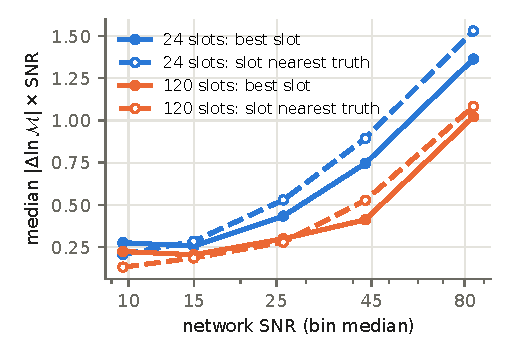
\includegraphics[width=\columnwidth]{bank_floor.pdf}
\caption{Chirp-mass error of the template bank alone, times SNR, for the best slot (solid) and the slot nearest the true mass ratio and spin (dashed), 3000 held-out BBH signals. A data-limited estimator is flat.}
\label{fig:bankfloor}
\end{figure}

\section{Discussion} \label{sec:discussion}

\subsection{Design principles}

Three choices run through the system and each is checked by a diagnostic
rather than assumed. The amplitude path is never normalized, because in
whitened strain amplitude is the distance cue; the distance correlation of
0.91 is the check. Overlaps are handled by rank conditioning rather than by
asking one context to describe every signal at once; the overlap-capacity test
is the check. And the objective is the NLL of Equation~\ref{eq:sbiobjective}
with a single auxiliary mass term; penalties on summary statistics of the
posterior (width, diversity) move those statistics without changing what the
context knows, which the shuffle statistic of Equation~\ref{eq:shuffle}
reveals. We report the shuffle statistic, coverage and SBC for every
checkpoint, because a network that trains without diverging has not
necessarily learned to condition on its input.

\subsection{Network and correction}

The network and the correction have different jobs. The network must have
reliable coverage and must cover every mode -- its widths set how much work the
correction has to do -- and it answers in seconds. The correction targets the
posterior under the exact likelihood, and its convergence is checked rather
than assumed (Section~\ref{sec:correction}). The real-event results show what
this division of labour buys: from a network posterior that is \pending{two to four
times} further from LVK than DINGO's network, the correction reaches the
accuracy of DINGO-IS. The sequential sampler's moves, not the proposal, carry
the particles onto the likelihood ridge, whereas single-step importance
sampling can only reweight what the network proposes. The cost of this
robustness is CPU time, minutes per event, and a residual weakness shared with
every importance-based method: relative weights of well-separated modes.

\subsection{Mass ratio and inclination}

Mass ratio and inclination are the parameters the network extracts least.
For inclination the reason is physical: the cross polarization scales as
$\cos\theta_{JN}$, so it carries information near edge-on and almost none near
face-on, and detected populations are dominated by face-on systems. Classifying
edge-on events ($|\cos\theta_{JN}|<0.3$, network SNR $\geq15$), the encoder's
matched-filter features reach an area under the ROC curve of 0.55, while
explicit cross-detector amplitude ratios and phase differences reach 0.72;
giving the classifier the true sky position and polarization in addition adds
nothing. The likelihood correction recovers the rest
(Section~\ref{sec:inclination}). For mass ratio, the correction with a
higher-mode likelihood is what matters on real heavy events: a dominant-mode
likelihood pushed GW190706 toward equal masses (LVK $q=0.52$, dominant-mode
0.90), and IMRPhenomXHM reduced the median mass-ratio offset across the O3
events from 0.35 to 0.12\,sd.

\section{Limitations} \label{sec:limits}

The network alone is broader than DINGO's network and leaves chirp-mass
information unused above SNR 35; the correction compensates, at minutes of CPU
time per event. Compared at equal SNR, the validation NLL of the BBH network is
\pending{0.8}\,nats worse in real than in Gaussian noise at SNR 10--20 and \pending{0.4} at
20--40, but \pending{4.0}\,nats worse at SNR 6--10, which the gate does not cover and
where much of the real-noise data lies.
Corrected distances on some events disagree with \texttt{dynesty} run on the
identical likelihood: for GW190412 (8\,s segment, LVK PSDs, IMRPhenomXHM)
\texttt{dynesty} gives a median of 671\,Mpc and the correction 776\,Mpc
(LVK: 690\,Mpc), while the masses agree. Since the setup is the same, this is a
convergence question for the correction, not a property of the likelihood, and
we are investigating it. Precession and detector calibration uncertainty are not modelled, and
\pending{primaries above $100\,\msun$ are outside the training prior [update if v9 is
adopted]}: the mass-ratio estimates for heavy events such as GW190602 and GW190706
lean toward equal masses in the network as well as the correction, because that prior holds no low mass
ratios at their chirp mass. Sky localization is limited when one detector dominates: GW190425 (L1 and a weak
V1) and GW200105 stay broad, and GW170817's depends on a gate the network never trained on. The most important unresolved inference problem is the weighting of
well-separated modes. For GW200115 the correction finds every part of the
posterior ridge but not their relative probabilities
(Section~\ref{sec:gw200115}); finding the modes is not enough if their weights
are wrong. The replicate test detects this and falls back to nested sampling,
which is correct but slow. The
network is trained for up to four overlapping signals and queries at most
five; the joint correction is validated against \texttt{dynesty} for two
\pending{[update after the three-signal tests]}. All overlap results here are on simulated
signals with stationary Gaussian noise; no overlapping signal has been analysed in real
data, so these results show the rank-conditioned network works in simulation, not that it
recovers overlaps in real observations.

\section{Future Work} \label{sec:future}

The bank probe points to a continuous refinement of the template estimate
along the chirp-mass--mass-ratio--spin ridge as the next step for loud-signal
precision; we are testing whether a local continuous search removes the
floor, and whether a network given that estimate can use it. A multi-peak
variant of the matched filter, which locates up to four signals by iteratively
subtracting the best template and gives each rank its own pivot, is in
training for overlapping segments, together with datasets of five to six
signals and a joint correction for three. A fifteen-parameter precessing model
is trained on a dedicated dataset. Marginalizing detector calibration
uncertainty and widening the BBH mass prior would bring the remaining catalog
misses into scope, and a larger real-noise bank with injected glitches is the
most direct attack on the Gaussian--real gap.

\section{Conclusion} \label{sec:conclusion}

LeanNPE turns the overlap problem into a well-posed query -- the posterior of
the $k$-th loudest signal -- answered by one network pass and corrected
against the exact likelihood by a tempered sequential Monte Carlo sampler.
\pending{[Numbers in this summary predate the 2026-11-05 fixes.]} Its BBH network has near-nominal marginal coverage in all eleven parameters in Gaussian and real
noise, matches \texttt{dynesty}'s chirp-mass width in the median on matched
injections, and keeps approximately nominal marginal coverage for up to four
overlapping signals in simulation; for two signals the joint correction agrees
with joint \texttt{dynesty} posteriors in under half an hour. On 28 O3 events
judged against the LVK posteriors, the correction turns a broad network
posterior into one with LVK-like widths and offsets of 0.17--0.36 LVK standard
deviations, comparable to DINGO-IS under the same noise spectra. Open problems
remain in the final posterior, not only in the network: relative mode weights
for multimodal events such as GW200115, and corrected distances that differ
from \texttt{dynesty} on some events. The network's remaining weakness,
chirp-mass precision on loud signals, survives encoder width, time alignment
and loss reweighting; a denser template bank helps, and a direct probe traces
the rest to the discreteness of the bank along the chirp-mass--mass-ratio--spin
degeneracy, which a continuous refinement should remove.

\section*{Acknowledgments}

This research made use of data, software, and web tools obtained from the
Gravitational Wave Open Science Center \citep{Vallisneri2015Gwosc,
Abbott2021Gwosc}, a service of LIGO Laboratory, the LIGO Scientific
Collaboration, and the Virgo Collaboration. This work used
\texttt{bilby} \citep{Ashton2019Bilby, Romero2020Bilby2},
\texttt{dynesty} \citep{Speagle2020Dynesty}, \texttt{nflows}
\citep{nflows}, \texttt{PyCBC} \citep{Harry2020PyCBC}, \texttt{PyTorch},
\texttt{gwpy}, and \texttt{Astropy} \citep{astropy}.

\software{bilby \citep{Ashton2019Bilby}, dynesty \citep{Speagle2020Dynesty}, nflows \citep{nflows}, PyCBC \citep{Harry2020PyCBC}, Astropy \citep{astropy}, PyTorch, GWpy}

\facility{LIGO, Virgo}

\bibliography{leannpe}
\bibliographystyle{aasjournalv7}

\end{document}
